% ----------------------------------------------------------------
% AMS-LaTeX Paper ************************************************
% **** -----------------------------------------------------------
\documentclass{amsart}
\usepackage{graphicx}

\graphicspath{{/Users/vynguyen/Google Drive/MathResearch (indiv)/Math Research Paper}}
% ----------------------------------------------------------------
\vfuzz2pt % Don't report over-full v-boxes if over-edge is small
\hfuzz2pt % Don't report over-full h-boxes if over-edge is small
% THEOREMS -------------------------------------------------------
\newtheorem{thm}{Theorem}[section]
\newtheorem{cor}[thm]{Corollary}
\newtheorem{lem}[thm]{Lemma}
\newtheorem{prop}[thm]{Proposition}
\theoremstyle{definition}
\newtheorem{defn}[thm]{Definition}
\theoremstyle{remark}
\newtheorem{rem}[thm]{Remark}
\theoremstyle{example}
\newtheorem{ex}[thm]{Example}
\theoremstyle{conjecture}
\newtheorem{conjecture}[thm]{Conjecture}
\numberwithin{equation}{section}
% MATH -----------------------------------------------------------
\newcommand{\norm}[1]{\left\Vert#1\right\Vert}
\newcommand{\abs}[1]{\left\vert#1\right\vert}
\newcommand{\set}[1]{\left\{#1\right\}}
\newcommand{\Real}{\mathbb R}
\newcommand{\eps}{\varepsilon}
\newcommand{\To}{\longrightarrow}
\newcommand{\BX}{\mathbf{B}(X)}
\newcommand{\A}{\mathcal{A}}
\newcommand{\lac}{\textit{lac }}
% ----------------------------------------------------------------
\begin{document}

\title{The Effect of Term Order on Identifying Models of Gene Regulatory Networks}%
\author{Brittani Boukather, Vy Nguyen, Pinky Patel, Brandilyn Stigler}%
%\address{}%
%\email{}%
%
%\thanks{}%
%\subjclass{}%
%\keywords{}%
%
%\date{}%
%\dedicatory{}%
%\commby{}%
% ----------------------------------------------------------------
\begin{abstract}
Gene regulatory networks (GRNs) control many life processes.  An
important problem in systems biology is to identify a model of the
network for a given set of laboratory data.  A recently developed
method builds a space of polynomial models from a given data set;
however, it requires that an order on the variables (genes) and an
order on the monomial terms (gene interactions) to be established.
No rigorous analyses have been performed to determine the impact of
these orders on the construction of the model space.

We chose a well-studied GRN in \textit{E. coli} to study the effect
of these orders on the identification of an existing model of the
network. We also determined how much data, as well as which data
explicitly are required for model identification.
\end{abstract}
\maketitle
% ----------------------------------------------------------------
\section{Introduction}

Gene regulatory networks (GRNs) are fundamental in orchestrating
life processes. Recent technology has allowed for amassing of large
amounts of data collected from probing GRNs. A growing problem is to
infer the network from the data. A recently developed method
constructs the space of polynomial models that fit the data. An
advantage of the model space is that it permits further analyses;
however, currently no extensive analyses have been performed. As the
modeling approach imposes an order on the variables (genes) and an
order on the monomial terms (gene interactions), rigorous analyses
will help to determine the impact of these orders on the
construction of the model space.

We highlight some results from exploring the relationship between
the data and the model space.  In particular we computed the size of
data sets necessary to guarantee a unique model in the space.
Additionally we identified which data sets specifically guarantee a
unique model.  As a consequence, we have established the hypothesis
that the choice of variable order has a greater impact on modeling
than the term order.  Solving this open problem will make
significant contributions towards refined experimental design and
more predictive models of GRNs.

In the following sections, we use the well-studied model of the \textit{lac} operon to determine the minimal size of data, and which data, are necessary to reversely engineer the correct model. We also look at the sufficiency of the data size, or more explicitly, the number of data which always guarantees the return of the correct model.

\section{Case Study: The \lac Operon}

The \lac operon is a network of genes that controls the
\textit{metabolism}, or breakdown, of lactose in \textit{E. coli}.

\begin{figure}
 \centering
    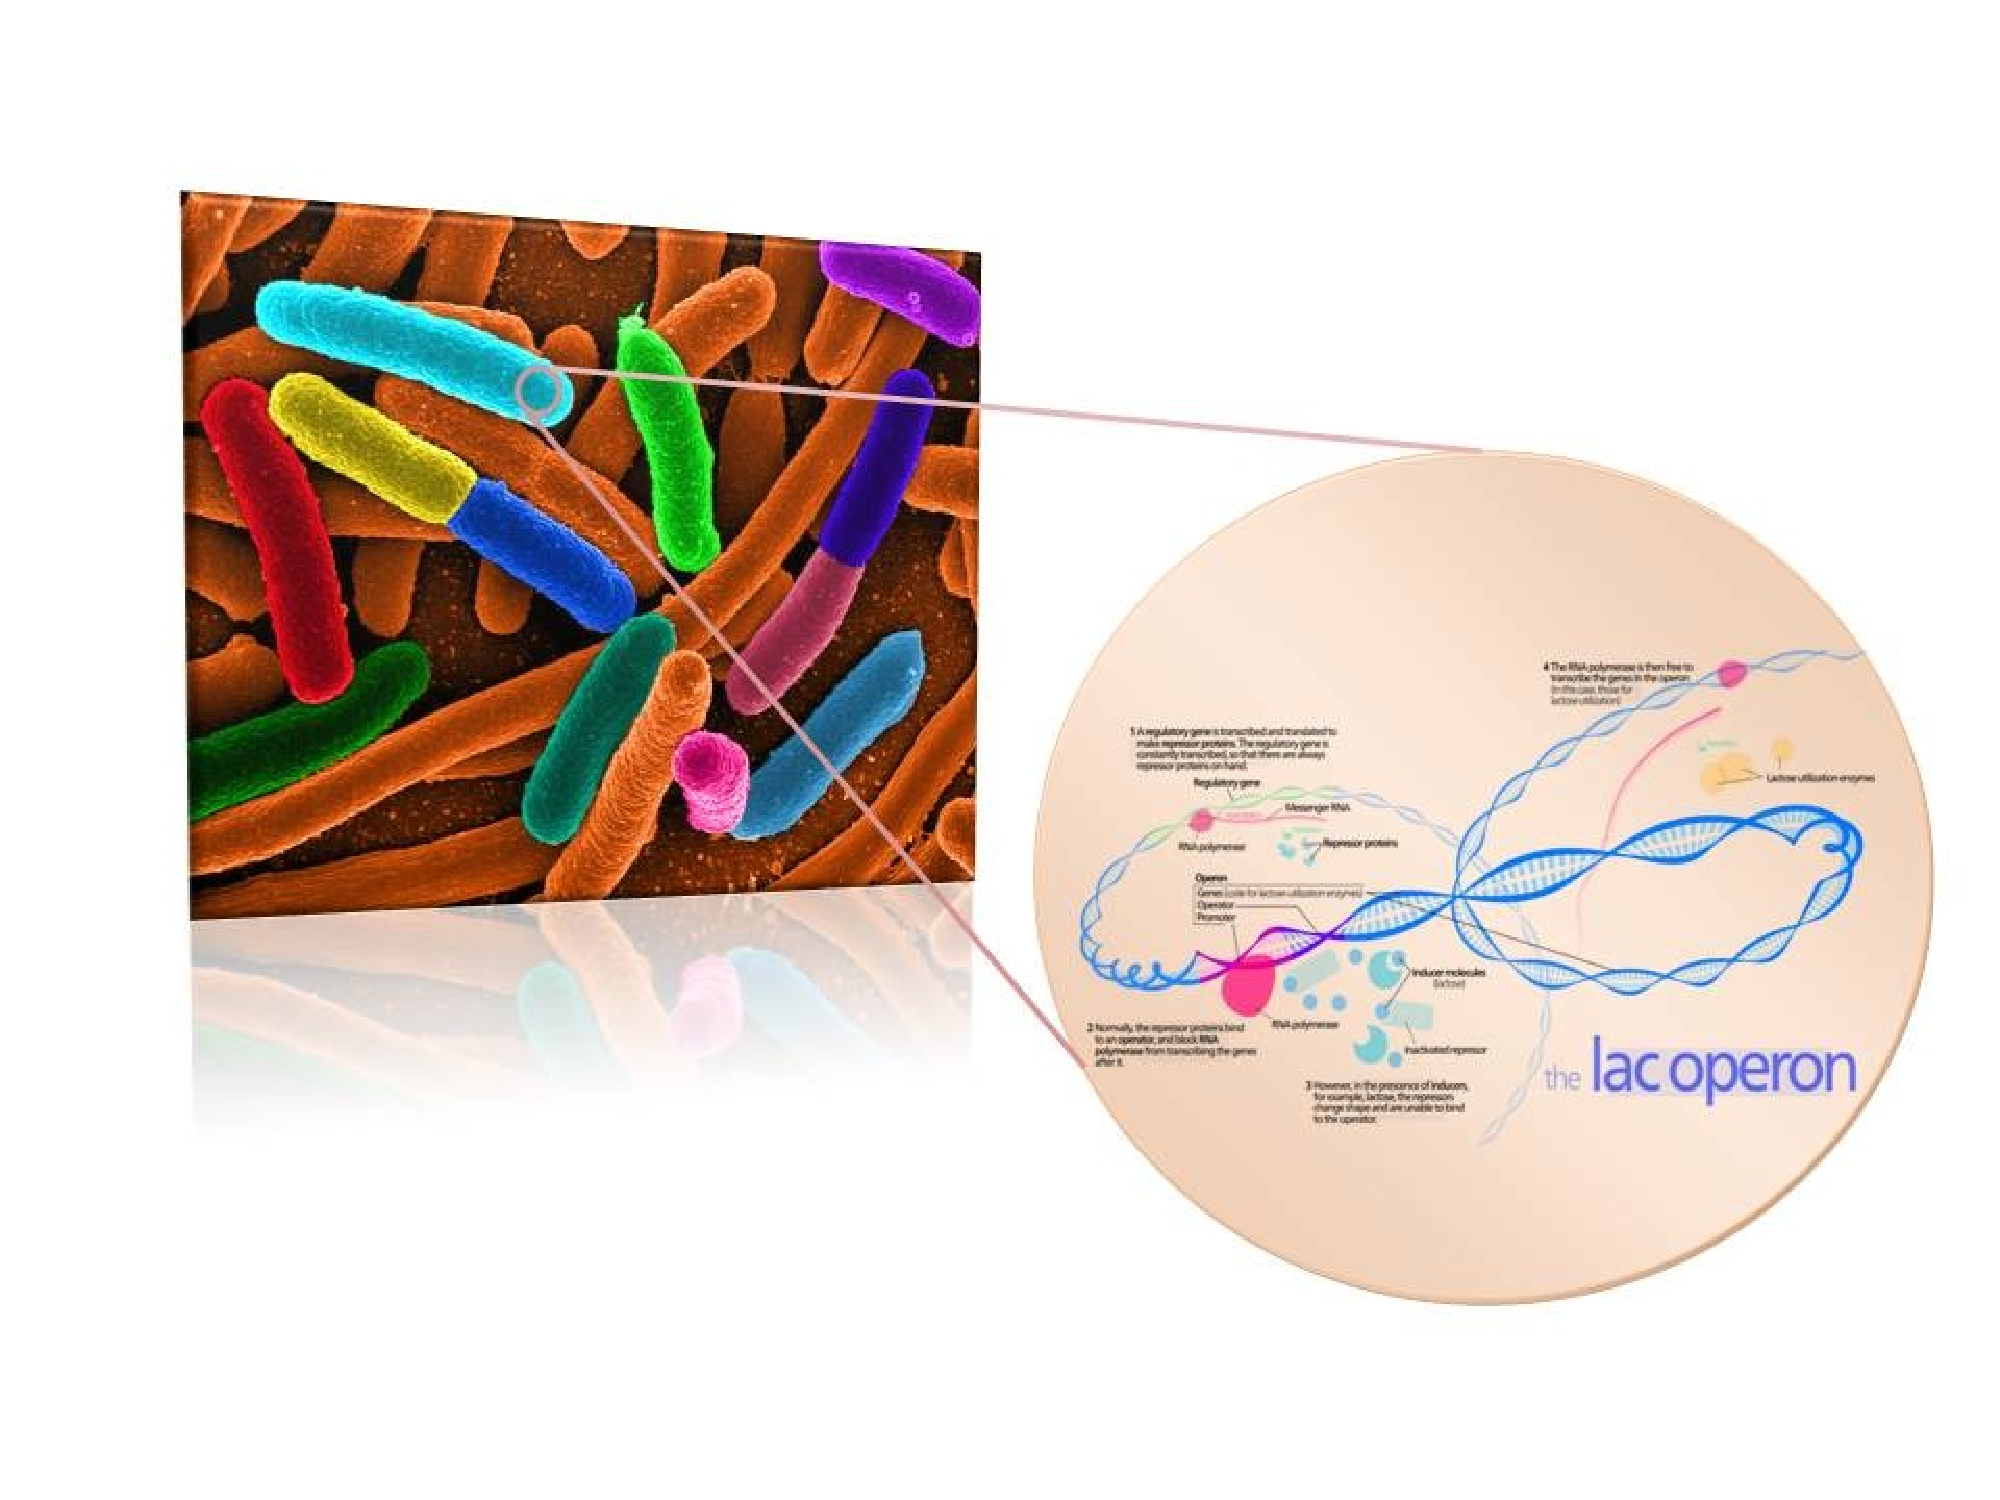
\includegraphics[scale=0.4]{lac.pdf}
  \caption{The \lac operon.}\label{}
\end{figure}

We used a simplified version of a published Boolean model of the
\lac operon \cite{veliz}, in which glucose concentrations are fixed.

\section{Preliminaries}
\subsection{Models of GRNs}
\label{sec-models}

A polynomial model for a GRN is a collection of polynomials, in
which the behavior of each gene is described by a polynomial
function.

The model for the \lac operon  is given by $F = (f_M , f_L , f_G)$
where
\begin{eqnarray*}
% \nonumber to remove numbering (before each equation)
  f_M &=& L \lor L_e \\
  f_L &=& M \\
  f_G &=& 1.
\end{eqnarray*}

Using the translation rules between Boolean functions and polynomial
functions
%
\begin{eqnarray*}
% \nonumber to remove numbering (before each equation)
  x\lor y &=& xy+x+y \\
  x\land y &=& xy \\
  \lnot x &=& x+1
\end{eqnarray*}
%
as well as the representation of $M, L, L_e, G$ with the variables
$x_1,x_2,x_3$ respectively, then the coordinate functions of $F$ can
be rewritten as
%
\begin{eqnarray}
\label{model}
 \nonumber %to remove numbering (before each equation)
  f_1 &=& x_2x_3+x_2+x_3 \\
  f_2 &=& x_1 \\
  \nonumber f_3 &=& 1
\end{eqnarray}
%
where each $f_i\in \mathbb Z_2[x_1,x_2,x_3]$.



\begin{figure}
  \centering
	 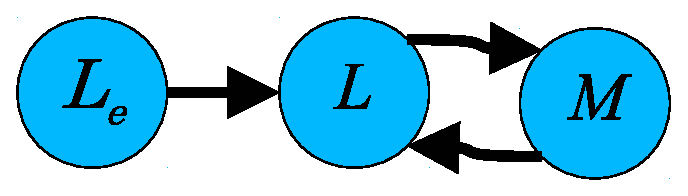
\includegraphics[width=1.5in]{wiring-diagram.eps}
  \caption{Wiring diagram of the model $F$.}\label{}
\end{figure}


We simulate the GRN by evaluating $F$ on all possible inputs.
\begin{figure}
  \centering
	 \includegraphics[scale=0.3]{state-space.pdf}
  \caption{The state space of the model $F$.}\label{}
\end{figure}


Probing a GRN typically produces incomplete data sets. It is a
problem to identify the model from these limited data.

\subsection{Model Building and Selection Using Algebraic Geometry}

The algebraic method in \cite{jarrah} computes all models that fit
given data.

We define the \textit{model space} to be the collection of functions
of the form $$F_p + F_h$$ where $F_p$ is a particular function that
fits the data, and $F_h$ is any     function that is zero on the
data. If $I = \{\text{all possible }F_h \}$, then
%
$$F_p \mod I : = \text{remainder of }F_p\text{ upon division by all
}F_h$$
%
is a ``minimal'' model that fits the data. However, polynomial
division is well defined only if $I$ is written as a Gr\"obner
basis.

All definitions are taken from \cite{cox}.

\begin{defn}
A \emph{Gr\"obner basis} is a multivariate nonlinear version of
Gauss-Jordan Elimination and requires a canonical way to write
polynomials.
\end{defn}

\begin{defn}
A \emph{variable order} (VO) is a sorting of variables, and a
\emph{monomial order}   (MO) is a rule for comparing monomials.  A
monomial order requires a variable order.
\end{defn}

\begin{ex}
If $x > y$, then $xy > y^3$  in lexicographic MO, \textit{i.e.}
dictionary order, while $y^3  > xy$ in graded lexicographic MO, in
which total degree is counted first.
    If $y > x$, then $y^3 > xy$ in both monomial orders.
\end{ex}

\section{Methods}
We considered all possible VOs on 3 variables (3! = 6). For each of
these VOs, we used the MOs \textit{lex}, \textit{glex}, and
\textit{grevlex}.  As $I$ is computed from data, we created all
subsets of the complete set of $2^3$ = 8 data points (see Section
\ref{sec-models}). We computed minimal models using each of the
$2^8$ = 256 subsets and reported which data sets, MOs, and VOs
result in the original model $F$.  The algorithms were executed in
\textit{Macaulay2} \cite{M2}.

\section{Results}

\begin{enumerate}
    \item Any subset of 7 data points is sufficient to return $F$.
    \item A minimum of 5 data points is necessary to return $F$.
    \begin{enumerate}
        \item Only 32 of the 56 possible subsets of 5 data points return $F$ (two such sets shown below).
        \item In these 32 subsets, each data point appears with  the same frequency (20).
    \end{enumerate}
    \item Each MO produced identical Gr\"obner bases, resulting in identical minimal models, though not always $F$.
    \item Only 2 VOs returned $F$.
\end{enumerate}

\begin{figure}
  \centering
  	\includegraphics[scale=0.3]{data1.pdf}\\
  \caption{Two sample data sets which return the model $F$.}\label{}
\end{figure}

\begin{figure}
  \centering
   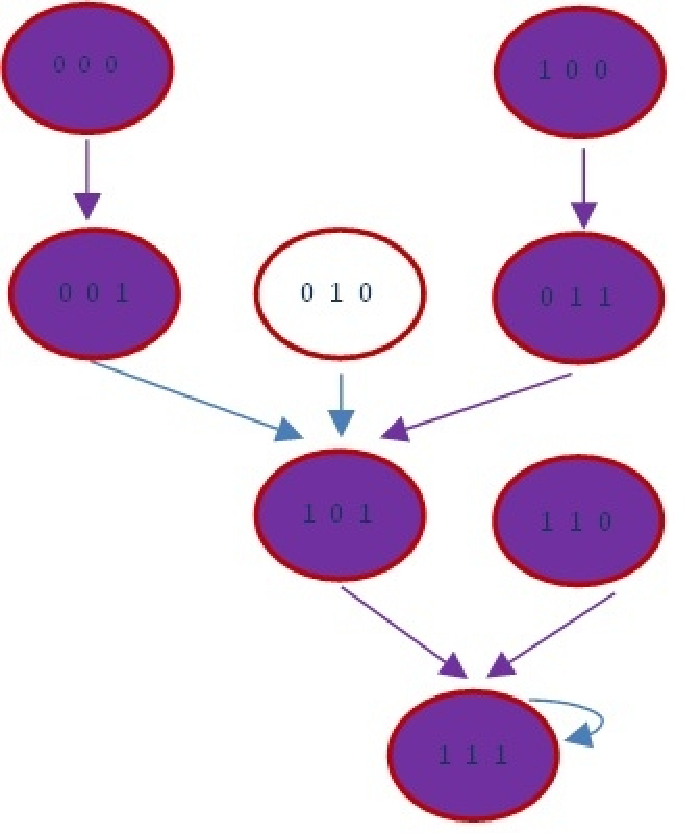
\includegraphics[scale=0.3]{data2.pdf}\\
  \caption{Two sample data sets which return the model $F$.}\label{}
\end{figure}

\section{Analysis}

\subsection {Identifying Minimal Data Size}
To understand why the model requires 5 points as the minimal data size, we will refer to the following result by Robbiano. 

\begin{thm}[Robbiano\cite{robbiano}]
\label{robbiano} $V\subseteq k^n$ identifies a polynomial $f$ if and
only if the evaluation matrix $X(V,f)$ has full rank.
\end{thm}

We will also need to define the support and closure of a polynomial.

\begin{defn}
Let $f$ be a polynomial.  The \emph{support} $s(f)$ of $f$ is the
collection of monomials $\{x^{\alpha_1},\ldots,x^{\alpha_m}\}$ that
appear in $f$. The \emph{closure} $\overline{s(f)}$ of $s(f)$ is the
set $\{x^{\beta} : x^\beta \mid x^{\alpha}, x^\alpha \in s(f)\}$ of
monomials that divide elements of $s(f)$. These monomials are also referred to as \emph{standard monomials}.
\end{defn}
Before we can prove the minimal data size for an F collection of polynomials, we need to look at the minimal data size for one polynomial f. 
\begin{lem}
\label{lem1} Let $f$ be a polynomial, $s(f)$ its support, and
$m=|\overline{s(f)}|$.  Then there exists $V\subseteq k^n$ that identifies f and m is the smallest integer such that $|V|=m$.
\end{lem}

\begin{proof}
Let $f$ be a polynomial and $s(f)$ its support.  Let
$m=|\overline{s(f)}|$.  Then there exists $V\subseteq k^n$ (could be all of $k^n$) such that $V$ identifies $f$.  By Theorem
\ref{robbiano}, $X(V,f)$ has rank $m\leq |V|$.  Since $X(V,f)$ is
potentially rectangular, we know we can find a square submatrix of
the same rank.  So there exists $V'\subseteq V$ such that $|V'|=m$.
Hence there is a subset $V'$ such that $X(V',f)$ has rank $m$ and
thus identifies $f$ by Theorem \ref{robbiano}.

To show that $m$ is the smallest such integer, suppose that there is
$W\subseteq k^n$ that identifies $f$ with $|W|<m$.  Then $X(W,f)$
has rank $m'$, which is strictly less than $m$.  Again, we can find
a square submatrix of rank $m'$.  However this means that one of the
monomials in $s(f)$ is not identified.  Hence, by Theorem
\ref{robbiano}, $W$ does not identify $f$, a contradiction
to the initial assumption.  Therefore, $m$ is the smallest such
integer.
\end{proof}

Now that we know the minimal data size for a single polynomial f is equal to the number of standard monomials, let's consider a system of polynomials $F={f_1,\dots,f_n}$ like the one we used for the\textit{lac} operon. We then have the following definitions. 

\begin{defn}
Let $F=(f_1,\ldots,f_n)$ be a PDS and $V=\{p_1,\ldots,p_m\}$ a
subset of point in $k^n$.  $V$ \emph{identifies} $f_i$ if the
coefficients of $f_i$ can be found uniquely by evaluation of the
monomials of $f$ on the points in $V$. Furthermore, $V$
\emph{identifies} $F$ if $V$ identifies each $f_i$.
\end{defn}

\begin{defn}
Let $F=(f_1, \ldots ,f_n)$ be a  polynomial dynamical system and
$V\subseteq k^n$. Let $X(V,f_1,\ldots,f_n)$ be the evaluation matrix
of the monomials in the support of each $f_i$ on the points in $V$.
In short, we write $X(V,F)$.
\end{defn}

We now try to extend Robbiano's result for a single polynomial to a system of polynomials.
\begin{thm}
\label{1}
$V\subseteq k^n$ identifies a polynomial dynamical system $F=(f_1,
\ldots ,f_n)$ if and only if the evaluation matrix $X(V,F)$ has full
rank.
\end{thm}

\begin{proof}
Let $V\subseteq k^n$, $F=(f_1, \ldots ,f_n)$ a PDS with $s(f_i)$
being the support of each $f_i$, and $m_i=|\overline{s(f_i)}|$.

Suppose $X(V,F)$ has full rank. Then $X(V,F)$ has full column rank. Since $m_i=|\overline{s(f_i)}|$,
then $X(V,f_i)$ has rank $m_i$.
%(So there is $V_i$ such that $X(V_i,f_i)$ has rank $m_i$).
So by Theorem \ref{robbiano}, $V$ identifies $f_i$. By definition,
$V$ identifies $F$.

Suppose $V$ identifies $F$.  So $V$ identifies each $f_i$.  So by
Theorem \ref{robbiano}, $X(V,f_i)$ has rank $m_i$.  Since
$\overline{\bigcup s(f_i)}$ contains $m$ linearly independent
monomials (as they are standard monomials), then the rank of
$X(V,F)= m$.
\end{proof}

Using the above theorem, we can now prove that the smallest size of V is equal to the number of standard monomials in F.

\begin{thm}
\label{thm2}
Let $F=(f_1,\ldots,f_n)$ be a PDS, $s(f_i)$ the support
of each coordinate function $f_i$, and $m=\lvert
\overline{\bigcup_{i=1}^n s(f_i)}\rvert$. Then there exists $V\subseteq k^n$ that identifies F and m is the smallest integer such that $|V|=m$.
\end{thm}

\begin{proof}
Suppose $F=(f_1,\ldots,f_n)$, $s(f_i)$ the support of each $f_i$,
$m=\lvert \overline{\bigcup_{i=1}^n s(f_i)}\rvert$, and
$m_i=|\overline{s(f_i)}|$. So $s(f_i)\subseteq
\overline{\bigcup_{i=1}^n s(f_i)}\rvert$, implying that $m_i\leq m$.
By Lemma \ref{lem1}, there exists $V_i$ such that $m_i$ is the
smallest integer where $V_i$ identifies $f_i$ and $|V_i|=m_i$.  Let
$V=\bigcup_{i=1}^n V_i$.  By construction, $V$ identifies $F$ since
a subset of $V$ identifies $f_i$.
%It follows that $|V|=|\bigcup V_i| \leq \sum |V_i| = \sum m_i$.
If $|V|=m$, then we are done.  Suppose $|V|<m$.  Then $X(V,F)$ has
rank $m'$, which is strictly less than $m$. But by Theorem
\ref{thm1}, if $V$ identifies $F$, then $X(V,F)$ must have rank $m$,
a contradiction.  Now suppose that $|V|>m$. So we can find
$V'\subset V$ such that $X(V',F)$ has rank $m$.  By Theorem
\ref{thm1}, $V'$ identifies $F$.

To show that $m$ is the smallest such integer, suppose that there is
$W\subseteq k^n$ that identifies $F$ with $|W|<m$.  Then $X(W,F)$
has rank $m'$, which is strictly less than $m$.  Again, we can find
a square submatrix of rank $m'$.  However this means that one of the
monomials in $s(f)$ is not identified.  Hence, by Theorem
\ref{1}, $W$ does not identify $F$, clearly a contradiction to
the initial assumption.  Therefore, $m$ is the smallest such
integer.
%Then $m$ is the smallest integer such that there exists $V\subset
%k^n$ such that $|V|=m$ and $V$ identifies $F$.
\end{proof}

Returning to our case study of the \textit{lac} operon model, since F has \emph{closure} $\overline{s(f)}$ = $\{1, x_1, x_2, x_3, x_2x_3\}$ and $|\overline{s(f)}| = 5$, then 5 data points are necessary to identify the model.


%[WHERE DO I PUT THESE 3]
%\begin{cor}[Cox 2]Any $f\in k[x]/I(V)$ is a linear combination of the standard monomials.
%\end{cor}
%\begin{prop}[Cox 2 Thm 2.10]If $V$ is a finite set of $m$ points, then the number
%of standard monomials equals $m$.
%\end{prop}
%\begin{prop}[Cox \cite{cox}]The minimal number of data points necessary to identify a normal form $f$
%equals the number of unique monomials that divide any term in $f$.
%[I DON'T THINK WE NEED THIS PROPOSITION]
%\end{prop}


\subsection{Identifying the Sufficient Data Set}
As $x_2x_3$ is the only mixed term, it follows that the pairs of
points

%\begin{table}
\begin{center}
\begin{tabular}{|c|c|c|c|}
  \hline
  % after \\: \hline or \cline{col1-col2} \cline{col3-col4} ...
  (1,6) & $d_1$ & 000 & 100 \\
  (2,3) & $d_2$ & 001 & 101 \\
  (5,8) & $d_3$ & 010 & 110 \\
  (7,4) & $d_4$ & 011 & 111 \\
  \hline
\end{tabular}
\end{center}
%  \caption{}\label{}
%\end{table}
%
all keep $x_2$ and $x_3$ fixed. So any function involving $x_2$ or
$x_3$ can be minimally described as a function of $x_2$ (if
$x_2<x_3$) or $x_3$ (if $x_3<x_2$)  but not $x_2x_3$.  That is
$x_2x_3$ is never smaller than $x_2$ or $x_3$ in any term order.


Data sets of size 5 with two of the above pairs never result in
normal forms containing $x_2x_3$. In fact, using any of these pairs
to build a data set results in reduced frequency (of appearing as a ``viable'' set.


\begin{lem}
Any data set of size 5 containing 2 of the above pairs will not
identify $F$.
\end{lem}

\begin{proof}
Consider a data set of size 5 with 2 pairs.  The evaluation matrix

$$A=
  \begin{array}{c|ccccc}
     & x_2x_3 & x_2 & x_3 & 1 & x_1 \\
     \hline
    p_{1,1} & a_1 & a_2 & a_3 & a_4 & * \\
    p_{1,2} & a_1 & a_2 & a_3 & a_4 & * \\
    p_{2,1} & b_1 & b_2 & b_3 & b_4 & * \\
    p_{2,2} & b_1 & b_2 & b_3 & b_4 & * \\
    d5 & * & * & * & * & * \\
  \end{array}$$

will have rank at most 4, where the starred entries can be either 0
or 1. Let $A_4$ be the $(4\time 4)$-matrix consisting of the first 4
rows and columns of $A$.  The first two rows of $A_4$ are equal and
so they contribute at most 1 pivot. So one of the first two entries
of the last column of $A$ can contribute 1 pivot in the row not
containing a pivot from $A_k$. Similarly, the last two rows of $A_4$
contribute at most 1 pivot. In this case, the third and fourth
entries of the last column of $A$ cannot contribute any pivot if
there is one already in one of the first two entries of the last
column of $A$. Finally, the last row of $A$ can contribute a pivot
in a column not containing one. Hence there are at most 4 pivots in
$A$, meaning any such data set does not identify $F$.
\end{proof}


There are ${4 \choose 2}=6$ data sets of size 4 containing two of
the above pairs.  There are 4 choices for the fifth point, resulting
in $6\times 4=24$ data sets that do not identify $F$.  As there are
${8 \choose 5}=56$ total sets of size 5, this leaves $56-24 = 32$
data sets of size 5 that identify $F$.  Note that all data
sets of size 5 will contain at least of the above pairs; however
data sets containing two pairs do not identify the model.

Can we generalize which data sets are necessary?
\begin{conjecture}
Any function containing a mixed term gives rise to a
collection of points that reduces the likelihood of a set containing
the collection to identify the PDS.  The number of points in the
collection is equal to the number of variables in the mixed term.
\end{conjecture}

\begin{conjecture}
Any function containing a mixed term gives rise to pairs
of points that reduces the likelihood of a set containing the
collection to identify the PDS.  These pairs hold two of the
variables in the mixed term fixed.  As such, any evaluation matrix
involving enough of these pairs will not have full rank (sub-rows
will be equal).
\end{conjecture}

Suppose $xy$ divides some mixed term.  This gives rise to a
collection of pairs of points that keep $xy$ fixed. %(4 such pairs?).
For every pair, we need an additional column in the evaluation
matrix in order to permit full rank.  So $n\geq 4+p$ where $p$
equals the number of pairs used to construct the evaluation matrix.

\begin{defn}
The data points $p$ and $q$ \emph{fix} a monomial $xy$ if
$x(p)=x(q)$ and $y(p)=y(q)$.  We call $(p,q)$ a pair that fixes
$xy$.
\end{defn}

Consider the submatrix corresponding to the rows for a pair $(p,q)$
and the columns associated to the monomial $xy$, that is the columns
for $xy$, $x$, and $y$.

$$\begin{array}{c|ccc}
     & xy & x & y\\
     \hline
    p & * & * & * \\
    q & * & * & * \\
  \end{array}
$$

Call the row associated to the point $p$ containing the entries from
the columns associated to $xy$, $x$, and $y$ the \emph{row for $p$}.

\begin{lem}
If $p$ and $q$ are not a pair that fixes a monomial $xy$, then the
row for $p$ does not equal the row for $q$.
\end{lem}

\begin{proof}
Let $p$ and $q$ not form a pair that fixes the monomial $xy$.  By
way of contradiction, suppose that the row for $p$ equals the row
 for $q$.  Then $xy(p)=xy(q)$, $x(p)=x(q)$, and $y(p)=y(q)$.  The
 last two equalities satisfy the definition of $p$ and $q$ being a
 pair, contradicting the hypothesis.  Hence, the
row for $p$ does not equal the row for $q$.
\end{proof}

So why are 7 data points sufficient? %Can we generalize?

Consider the full evaluation matrix on 8 data points.  

$$A=
  \begin{array}{c|cccccccc}
     & x_1& x_2 & x_3 & x_1x_2 & x_2x_3 & x_1x_3 &1 & x_1x_2x_3 \\
     \hline
    p_{1,0,0} & 1 & 0 & 0 & 0 & 0 & 0 & 1 & 0 \\
    p_{0,1,0} & 0 & 1 & 0 & 0 & 0 & 0 & 1 & 0\\
    p_{0,0,1} & 0 & 0 & 1 & 0 & 0 & 0 & 1 & 0 \\
    p_{1,1,0} & 1 & 1 & 0 & 1 & 0 & 0 & 1 & 0 \\
    p_{0,1,1} & 0 & 1 & 1 & 0 & 1 & 0 & 1 & 0 \\
    p_{1,0,1} & 1 & 0 & 1 & 0 & 0 & 1 & 1 & 0 \\
    p_{0,0,0} & 0 & 0 & 0 & 0 & 0 & 0 & 1 & 0 \\
    p_{1,1,1} & 1 & 1 & 1 & 1 & 1 & 1 & 1 & 1 \\
  \end{array}$$
  
%\begin{proof}
%Show that all $(7\times 7)$-matrices have full rank (this has been
%checked in our case and is true). We know that the column
%corresponding to $x_1x_2x_3$ must be deleted. So the resulting
%$(8\times 7)$-matrix has rank $\leq$ 7 (What is the min possible
%rank from removing a single column or row?). If it has rank 7 (which
%it does), this means that the 7 cols are LI and there exist 7 rows
%which are LI. Is it the case that all $(7\times 7)$-submatrices have
%rank 7? Or why is the case for us?
%\end{proof}


Consider the following analysis on pairs:

Specific to our model: Consider a data set of 3 pairs and one
additional point.  In a pair, the rows must differ at $x_1$;
otherwise the two points are the same. The rows for two points not
being a pair must differ on $x_2$ or $x_3$; else the points form a
pair. The row for a 7th point $p$ must differ with all other rows of
points; otherwise $p$ would form a triple with an existing pair,
which is not possible.


\textbf{Claim}: the evaluation matrix with last column removed and any row
removed has full rank ($2^n-1$).

%Does every square matrix with a column and a row of 1s and distinct
%rows and columns have full rank?

If the number of monomials of degree $d$ in the model is less than
or equal to the total number of possible monomials of degree $d$,
then the \\
\centerline{
Sufficiency number $=min$((total number of mons up to degree $d$) +
1, $2^n-1$)}






\section{Discussion}

The results suggest that the choice of  variable order has a greater
impact on identifying models than the monomial order. Solving this
open problem will make significant contributions towards refined
experimental design and more predictive models of GRNs. To test the
validity of the new hypothesis, further studies of monomial orders
and models of higher degree will be conducted.


\bibliography{references}
\bibliographystyle{amsplain}
\end{document}

